\chapter{%
実験}

RGB-Dカメラから取得したデータセットをRXDネットワークを使用し曲管又はT字管を認識できるか検証する。
物体認識においては他のネットワークでも実験し、RXDネットワークの有用性を確かめる。
また、物体検出から得た情報を元に姿勢推定も行う。

\section{評価指標}
物体認識の評価指標ではパラメータ数(Params), Intersection over Union(IoU), mean Average Precision(mAP)を用い認識ネットワークの性能評価を行う。
まず、パラメータ数は認識ネットワークの学習可能なパラメータの合計数を示す。これにより、認識ネットワークの複雑度を示すことができ、パラメータ数が多いほどネットワークが複雑になり推論字管が長くなるのが一般的である。
次に、IoUは図4.1のように正解ラベルと予測のバウンディングボックスの共通の重なり部分と、2つのバウンディングボックスを重ねたときの総面積で除算したものである。
IoUは0~1.0の値の範囲で示され、値が大きければ大きいほどラベル付されたボックスと予測されたボックスの重なりが正しいことになり、正確に認識していると判断できる。
次に、mAPは一つ一つのクラスに対して平均適合率であるAP(Average Precision)を計算する。まず、モデルの予測結果を、出力する信頼度スコア順に並べる。
ラベルごとに信頼度スコアがそのラベルの値以上の予測結果について、適合率と再現率を求める。適合率と再現率は図4.2のようにTrue Positive(TP)とFalse Negative(FN)を用いて表される。
その適合率と再現率のグラフから適合率の下側の面積を求める。ここで、予測されたラベルが正解なのかの判断はIoUが決められたしきい値以上で、最も信頼度スコアが高い予測ラベルが正解とするように判断される。
そして最後に、クラスごとに計算されたAPの平均を算出したものがmAPになる。APはIoUの閾値によって認識条件の厳しさが変わるため、
本研究におけるAPの評価方法はIoUの閾値を0.5にしたものをAP50にし、IoU閾値を0.5から0.95の間で0.05ずつ上昇させて求められた結果を平均したものをAPとして検証する。
また、物体検出におけるクラス分けは曲管をbentにし、T字管をjunctionとして設定した。
\begin{figure}[htbt]
	\centering
	 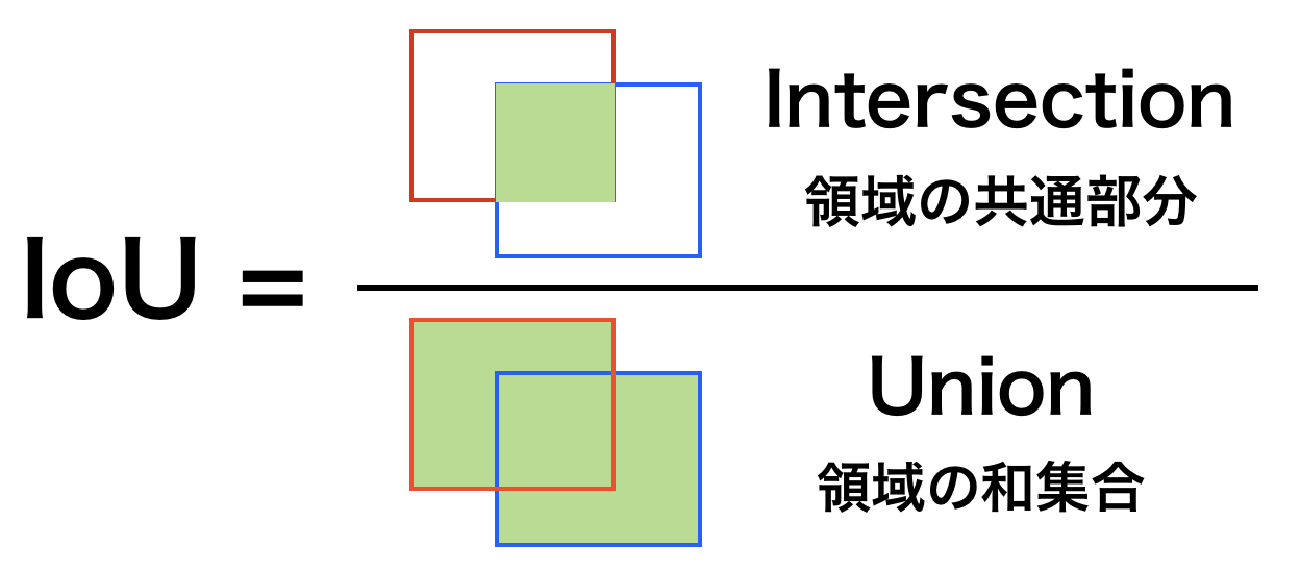
\includegraphics[height=53mm]{iou.eps}
	 \caption{Intersection over Union(IOU)}
	 \label{fig:f2}
\end{figure}

\begin{figure}[htbt]
	\centering
	 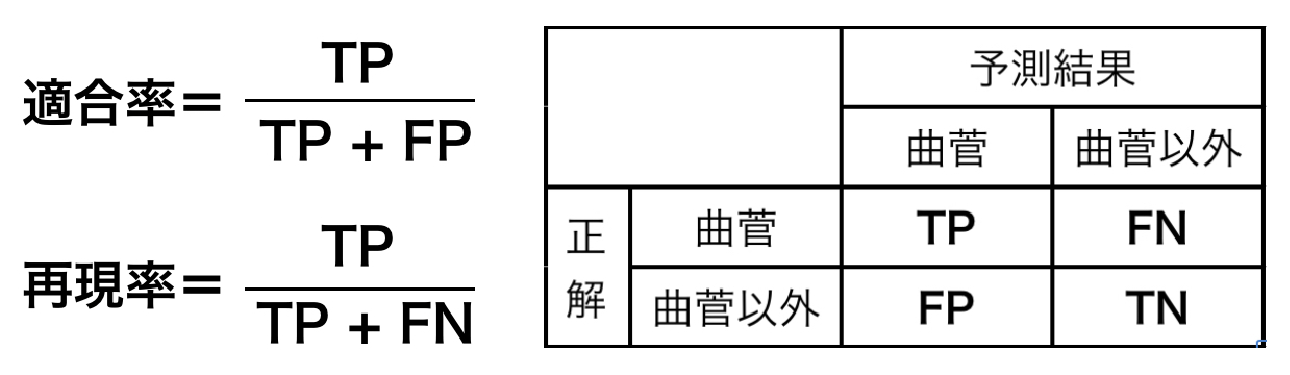
\includegraphics[height=40mm]{recall.eps}
	 \caption{適合率と再現率}
	 \label{fig:f2}
\end{figure}


\section{結果と考察}
\subsection{物体検出}
表4.1,図4.3,図4.4より、RXDネットワークがmAPとmAP50の平均値がともに最も数値が高い結果を示した。APの値が高いほど配管の認識精度が良いことを示しているため、YOLOv3とYOLOv3-DepthよりもRXDネットワークのほうが優れた精度を発揮すると言える。
しかし、APの平均値はともにRXDが優れた結果になったが、bentとjunction個々のAP値で見るとYOLOv3のほうがjunctionを検出するにおいて良い結果を示した。そのため、認識したい物体がT字管のみを検出する場合にはRXDよりもYOLOV3のほうが認識精度は良くなると考えられる。
また、評価指標はmAPとmAP50で行ったが、どのネットワークにおいてもmAPのほうがmAP50よりも精度が悪い結果となった。これはmAPの方は閾値を0.5~0.95の間で0.05刻みでIoUの閾値を上昇させているため、重なり合う面積の大きさの条件をより厳しくしているからだ。
IoU閾値を増加させても認識精度が低くならないネットワークが優秀とされているが、今回の結果においてはどのネットワークも精度が大きく落ちているため、ネットワーク改善を行う必要性があると考えられる。\\
次に、パラメータ数に関してはYOLOv3, YOLOv3-DepthよりもRXDは低い値を示している。パラメータ数が高いとネットワークの構造が複雑になることを示しているため、推論時間も比例して長くなる。そのため、RXDは他のネットワークよりも認識結果を
より速く示すことが期待できる。
一方、YOLOv3とYOLOv3-Depthのパラメータ数を比較すると1.4倍ほど差が存在している。YOLOV3-DepthはDepth画像を使用していることからデータセットの量はYOLOv3よりも2倍になるため、ネットワークは必然的に畳み込みむ回数が増加し
パラメータ数が結果的に多くなることを意味している。そのため、RXDはYOLOv3-Depthと同様にDepth画像を用いていることからパラメータ数が多くなることが予測できるがYOLOv3よりもパラメータ数が低い結果を示した。
RXDはネットワーク設計段階で畳み込み層の回数の調整や出力チャネルの削減、RXD層の効果的なRGB画像とDepth画像の特徴共有を達成していることがパラメータを数削減しながらも安定した精度を出力する結果につながっていると考えられる。\\




\clearpage

\begin{table}[htbp]
\centering
\caption{物体検出ネットワークの実行結果}
\resizebox{\textwidth}{!}{%
\begin{tabular}{llllllll}
\hline
	\textit{\textbf{}} & \textit{\textbf{}} & \textit{\textbf{mAP}} & \textit{\textbf{}} & \textit{\textbf{}} & \textit{\textbf{mAP50}} & \textit{\textbf{}} & \textit{\textbf{Parameters}} \\
\textit{\textbf{Network}} & \textit{\textbf{bent}} & \textit{\textbf{junction}} & \textit{\textbf{mean}} &  \textit{\textbf{bent}} & \textit{\textbf{junction}} & \textit{\textbf{mean}} & \textit{\textbf{}} \textit{\textbf{millions}} \\ \hline
YOLOV3              & 33.9                 & 68.6                                 & 51.3                      & 9.95                      & 20.1                          & 15.0                     & 61.5                                \\
YOLOV3-Depth        & 1.3                  & 0.0                                 & 0.7                      & 0.4                      & 0.0                          	& 0.2                     & 86.3                                	\\
RXD                 & 70.9                 & 37.2                                 & 54.1                      & 20.8                      & 10.9                          & 15.8                     & 32.4                                 \\
\end{tabular}%
}
\end{table}

\begin{figure}[htbt]
	\centering
	 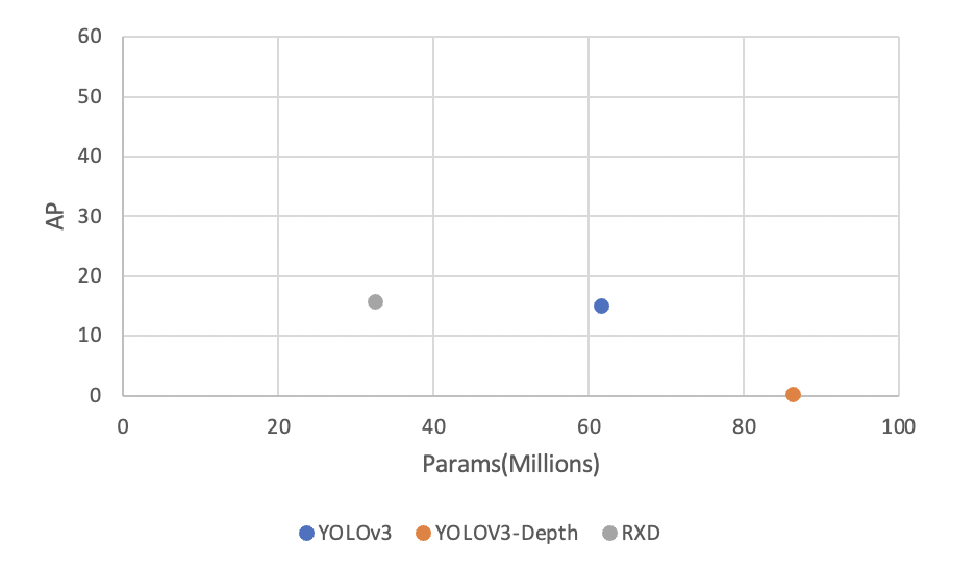
\includegraphics[height=70mm]{ap.eps}
	 \caption{mAPによる検出結果}
	 \label{fig:f2}
\end{figure}

\begin{figure}[htbt]
	\centering
	
	 \includegraphics[height=70mm]{ap50.eps}
	 \caption{mAP50による検出結果}
	 \label{fig:f2}
\end{figure}

\newpage

\begin{figure}[htbt]
	\centering
	 \includegraphics[height=95mm]{re0.eps}
	 \label{fig:f2}
\end{figure}

\begin{figure}[htbt]
	\centering
	 \includegraphics[height=95mm]{re1.eps}
	 \caption{各ネットワークの検出結果}
	 \label{fig:f2}
\end{figure}

\newpage

\clearpage

図4.5にはRGB-Dカメラから得られたRGB画像とDepth画像、曲管やT字管のラベリングを行ったGround Truth画像、各ネットワークの検出結果をそれぞれ示した。結果より正解ラベルと最も近しい検出結果を示したのはRXDネットワークであると言える。
しかし、RXDネットワークの出力されたデータにはT字管を認識できていない結果も存在している。これは、もとのDepth画像のデータセットを参考にすると遠くの物体になるほどデータが欠落していることが図中の3番の画像からわかる。
そのため、他のデータセットにおいてもカメラに近いオブジェクトが認識できても遠距離になるにつれて認識精度が悪くなる結果になった。
よって、精度がより好ましいRGB-Dカメラを使用することや、Depth画像取得の際にフィルタリングでデータの欠落を埋める作業を取り入れる必要性がある。\\
 また、図中の4番のテスト画像では暗闇の状況下での検出を試みた結果、YOLOv3-DepthとRXDネットワークの出力がうまく配管を検出できていた。
これは暗闇の状況下でも影響を受けないDepth画像が推論において役に立っていると考えられ、RGB-Dカメラの有効性を示すことができたと言える。

\begin{figure}[htbt]
	\centering
	 \includegraphics[height=120mm]{6d.eps}
	 \caption{適合率と再現率}
	 \label{fig:f2}
\end{figure}

次に、6D姿勢推定の結果を図4.6に示す。既存のGen6Dのみでは検出器がオブジェクトの複数認識に対応していなかった。RXDネットワークは画像の中の全てのオブジェクトを認識可能なため、検出された値をGen6DのSelectorに渡すことで複数姿勢推定を可能とする。
しかし、結果では曲管の姿勢がボックスとうまく一致しなく望ましくない結果になったが比較的安定した姿勢推定が行えていると判断できる。

\begin{table}[htbp]
\centering
\caption{物体検出ネットワークの実行結果}
\resizebox{\textwidth}{!}{%
\begin{tabular}{llllllll}
\hline
\textit{\textbf{Junction1(left)}} & \textit{\textbf{Junction2(right)}} \\ \hline
Yaw         & -2.453460 &  0.7020501        \\
Pitch				&	0.0145083	 &	0.0262553			\\
Roll        & 1.7120977  & 1.6288774    \\
\end{tabular}%
}
\end{table}

\begin{figure}[htbt]
	\centering
	 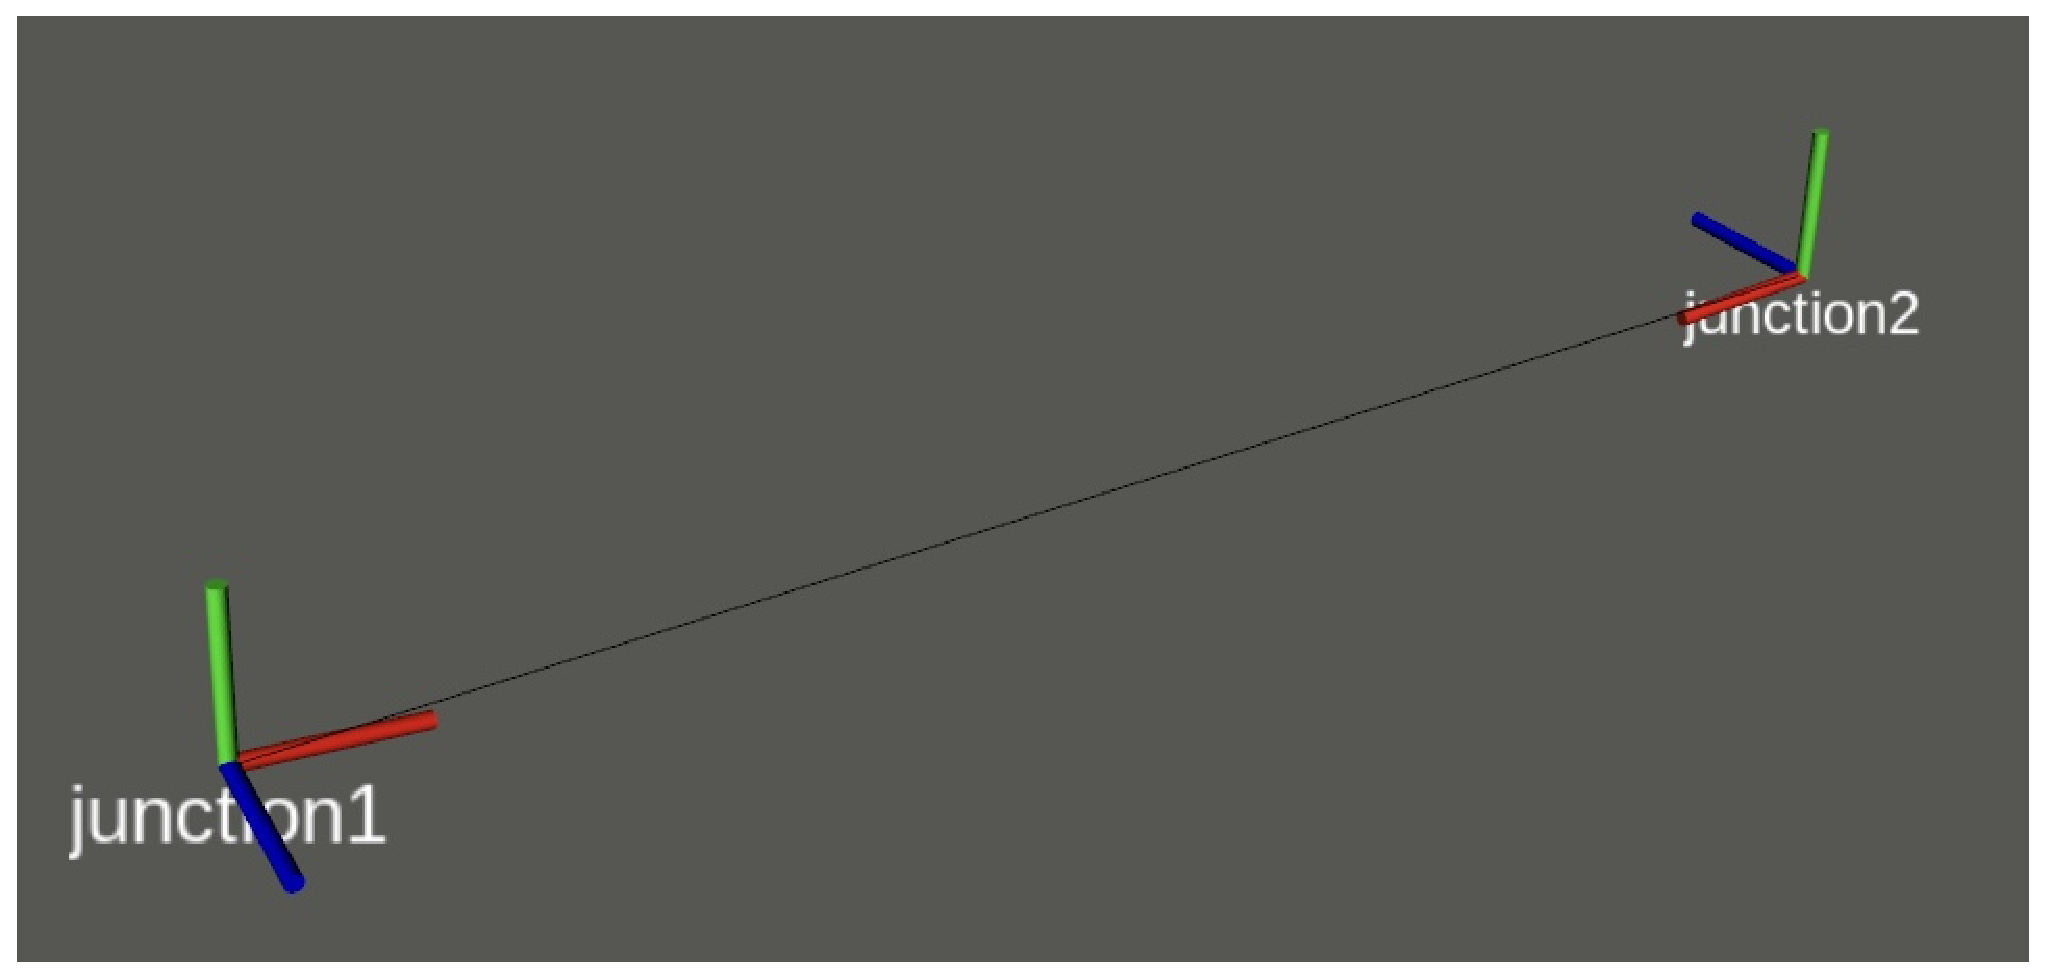
\includegraphics[height=65mm]{rviz.eps}
	 \caption{Rvizを用いたT字管の座標系の可視化}
	 \label{fig:f2}
\end{figure}

また、図4.6の1番の画像のようにjunction同士が向かい合っている画像の姿勢推定より、それぞれのオブジェクトのYaw, Pitch, Rollを求めた。表の結よりjunction同士が向かい合っていることがわかる。
Gen6Dは認識したオブジェクトに対して回転行列と移動ベクトルを出力する。その結果を元にYaw, Pitch, Rollを算出した。その結果は表4.2のようになり、それぞれの値を用いて、図4.7のようにRvizを使用して
それぞれのオブジェクトの座標系を可視化した。座標系を求められたことで完全に向かい合った結果にはならなかったが、T字管の位置関係と姿勢を表示することができた。

\begin{figure}[htbt]
	\centering
	 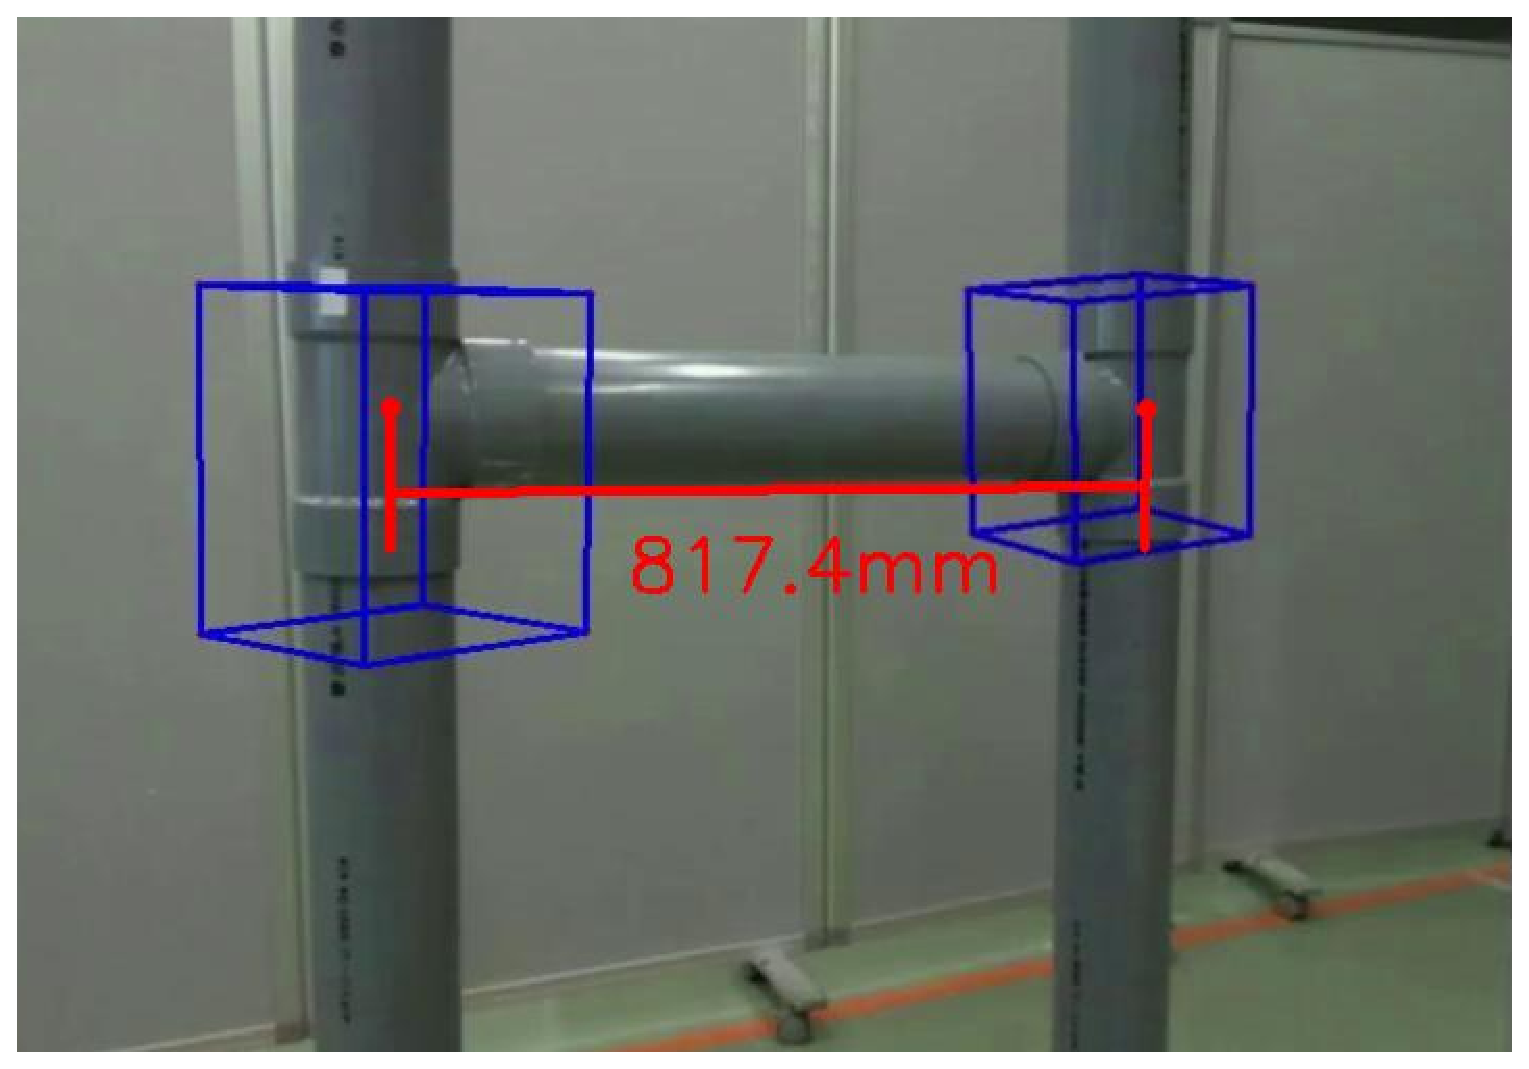
\includegraphics[height=85mm]{scale.eps}
	 \caption{算出されたT字管の距離}
	 \label{fig:f2}
\end{figure}

\begin{figure}[htbt]
	\centering
	 \includegraphics[height=85mm]{realscale.eps}
	 \caption{実際のT字管の距離}
	 \label{fig:f2}
\end{figure}

最後に、姿勢推定した結果からDepth画像を使用してT字管の間の距離測定を行う。姿勢推定した結果には距離情報を含んでいないため、推定されたオブジェクトのピクセル中心座標を深度画像と照らし合わせることでオブジェクト間の距離を算出する。
図4.7及び図4.8にそれぞれに実際の測定値と出力された結果を用いて算出された距離情報の結果を示す。実際の距離が817.3mmだったのに対し、Depth画像によって求められたスケールは817.3mmであった。誤差は生じているが、Depth画像を用いることで
姿勢推定した結果に距離情報を与えることができていると言える。\\
以上の結果より、アイソメ図作成に必要な情報である曲管及びT字管の姿勢推定と距離情報を求められるプロセスを確立することができた。